
\chapter[Dạng bài: Quá trình biến đổi lực\\ của con lắc đơn chịu tác dụng\\ của ngoại lực]{Dạng bài: Quá trình biến đổi lực của con lắc đơn\\ chịu tác dụng của ngoại lực}
\section{Lý thuyết}
\subsection{Con lắc đơn chịu tác dụng của lực quán tính}
\begin{itemize}
	\item Lực quán tính được xác định theo biểu thức:
	\begin{equation*}
		\overrightarrow{F_{\text{qt}}} = - m \vec{a}
	\end{equation*}  
	\item Trọng lượng biểu kiến của con lắc trong thang máy:
	
	+ Con lắc đi lên nhanh dần đều (hoặc đi xuống chậm dần đều):
	\begin{equation*}
		g'=g+a \Rightarrow P' = mg' =m(g+a) \Rightarrow T = 2\pi \sqrt{\dfrac{l}{g+a}}.
	\end{equation*}
	
	+ Con lắc đi lên chậm dần đều (hoặc đi xuống nhanh dần đều):
	\begin{equation*}
		g'=g-a \Rightarrow P' = mg' =m(g-a) \Rightarrow T = 2\pi \sqrt{\dfrac{l}{g-a}}.
	\end{equation*}
	
	\item Con lắc chịu tác dụng của lực quán tính $\vec{F_{\text{qt}}} = - m \vec{a}$ theo phương ngang:
	\begin{equation*}
		g'=\sqrt{g^2+a^2} \Rightarrow P'=mg'=m\sqrt{g^2+a^2} \Rightarrow T=2\pi \sqrt{\dfrac{l}{g^2+a^2}}.
	\end{equation*}	 
\end{itemize}
\subsection{Con lắc đơn chịu tác dụng của lực điện trường}
\begin{itemize}
	\item Lực điện trường được xác định theo biểu thức:
	\begin{equation*}
		\vec{F}=q \vec{E}
	\end{equation*}
	\item Trường hợp 1: $\vec{E}$ có hướng thẳng đứng xuống dưới.
	
	+ Nếu $q <0$, khi đó $\vec{F}$ ngược chiều với $\vec{E}$ nên $\vec{F}$ hướng thẳng đứng lên trên.
	\begin{equation*}
		P'=P-F \Leftrightarrow g'=g - \dfrac{|q|E}{m}.
	\end{equation*}
	Chu kỳ dao động của con lắc khi đặt trong điện trường:
	\begin{equation*}
		T' =2\pi \sqrt{\dfrac{l}{g-\dfrac{|q|E}{m}}}.
	\end{equation*}
	+ Nếu $q >0$, khi đó $\vec{F}$ cùng chiều với $\vec{E}$ nên $\vec{F}$ hướng thẳng đứng xuống dưới.
	\begin{equation*}
		P'=P+F \Rightarrow g'=g + \dfrac{|q|E}{m}.
	\end{equation*}
	Chu kỳ dao động của con lắc khi đặt trong điện trường:
	\begin{equation*}
		T'=2\pi \sqrt{\dfrac{l}{g+\dfrac{|q|E}{m}}}.
	\end{equation*}
	\item Trường hợp 2: $\vec{E}$ có hướng thẳng đứng lên trên.
	
	+ Nếu $q <0$, khi đó $\vec{F}$ ngược chiều với $\vec{E}$ nên $\vec{F}$ hướng thẳng đứng xuống dưới.
	\begin{equation*}
		P'=P+F \Rightarrow g'=g + \dfrac{|q|E}{m}.
	\end{equation*}
	Chu kỳ dao động của con lắc khi đặt trong điện trường:
	\begin{equation*}
		T' =2\pi \sqrt{\dfrac{l}{g+\dfrac{|q|E}{m}}}.
	\end{equation*}
	+ Nếu $q >0$, khi đó $\vec{F}$ cùng chiều với $\vec{E}$ nên $\vec{F}$ hướng thẳng đứng lên trên.
	\begin{equation*}
		P'=P-F \Rightarrow g'=g - \dfrac{|q|E}{m}.
	\end{equation*}
	Chu kỳ dao động của con lắc khi đặt trong điện trường:
	\begin{equation*}
		T' =2\pi \sqrt{\dfrac{l}{g-\dfrac{|q|E}{m}}}.
	\end{equation*}
	
	\item Trường hợp 3: $\vec{E}$ có phương ngang.
	\begin{center}
		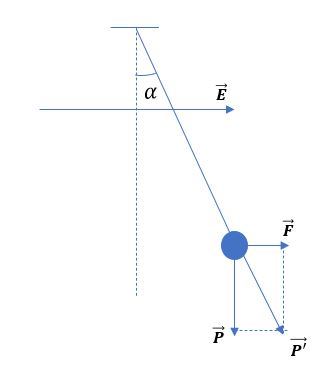
\includegraphics[scale=0.8]{../figs/VN12-PH-04-A-003-3-V2-1.JPG}
	\end{center}
	+ Do trọng lực $\vec P$ hướng xuống nên $\vec{F}$ vuông góc với $\vec{P}$, ta được:
	\begin{equation*}
		P'^2 =P^2+F^2 \Rightarrow g'=\sqrt{g^2 + (\dfrac{|q|E}{m})^2}.
	\end{equation*}
	+ Góc lệch của con lắc so với phương ngang (hay còn gọi là vị trí cân bằng của con lắc trong điện trường) được tính bởi:
	\begin{equation*}
		\tan \alpha =\dfrac{F}{P} = \dfrac{|q|E}{mg}.
	\end{equation*}
\end{itemize}
\section{Mục tiêu bài học - Ví dụ minh họa}
\begin{dang}{Xây dựng được công thức tính chu kì của con lắc đơn chịu tác dụng của ngoại lực}
	\viduii{3}
	{
		Một con lắc đơn được treo vào trần của một thang máy đang đứng yên tại nơi có gia tốc trọng trường $g=\text{9,9225}\ \text{m/s}^2$, con lắc đơn dao động điều hòa, trong thời gian $\Delta t$ con lắc thực hiện được 210 dao động toàn phần. Cho thang máy đi xuống nhanh dần đều theo phương thẳng đứng với gia tốc có độ lớn không đổi bằng $a = 180\ \text{cm/s}^2$ thì con lắc dao động điều hòa, trong thời gian $\Delta t$ con lắc thực hiện được bao nhiêu dao động toàn phần?
	}
	{
		\begin{center}
			\textbf{Hướng dẫn giải}
		\end{center}
		
		Thang máy đứng yên:
		\begin{equation*}
			\Delta t = N \cdot T = N \cdot 2\pi \sqrt{\dfrac{l}{g}}.
		\end{equation*}
		
		Thang máy xuống nhanh dần đều:
		\begin{equation*}
			\Delta t = N' \cdot T' = N' \cdot 2\pi \sqrt{\dfrac{l}{g'}} = N'\cdot 2\pi \sqrt{\dfrac{l}{g-a}}.
		\end{equation*}
		Suy ra:
		
		\begin{equation*}
			N \cdot 2\pi \sqrt{\dfrac{l}{g}} = N'\cdot 2\pi \sqrt{\dfrac{l}{g-a}}  \Rightarrow N' = 190\ \text{dao động}.
		\end{equation*} 
	}
	\viduii{4}
	{
		Một con lắc đơn có vật nhỏ mang điện tích dương được treo ở một nơi trên mặt đất trong điện trường đều có cường độ điện trường $\vec E$. Khi $\vec E$ hướng thẳng đứng xuống dưới thì con lắc dao động điều hoà với chu kì $T_1$. Khi $\vec E$ có phương nằm ngang thì con lắc dao động điều hoà với chu kì $T_2$. Biết trong hai trường hợp, độ lớn cường độ điện trường bằng nhau. Tỉ số $\dfrac{T_2}{T_1}$ có thể nhận giá trị nào sau đây?
		\begin{mcq}(4)
			\item 0,89.
			\item 1,23.
			\item 0,96.
			\item 1,15.
		\end{mcq}
	}
	{\begin{center}
			\textbf{Hướng dẫn giải}
		\end{center}
		
		Ta có $q>0$, khi $\vec E$ hướng xuống thì $\vec a$ hướng xuống. Suy ra:
		$$g_1 = g+a$$
		
		Khi $\vec E$ nằm ngang thì
		
		$$g_2=\sqrt{g^2 + a^2}$$
		
		Suy ra $$\dfrac{T_2}{T_1}=\dfrac{\sqrt{g_1}}{\sqrt{g_2}}=\dfrac{\sqrt{g+a}}{\sqrt{\sqrt{g^2+a^2}}}.$$
		
		Đặt $\dfrac{T_2}{T_1} = A$, ta có:
		$$1<A<\sqrt[4]{2} \Rightarrow 1 <\dfrac{T_2}{T_1} < 1,1892.$$
		
		Biến đổi $A^2$:
		$$A^2 = \dfrac{g+a}{\sqrt{g^2+a^2}}=\dfrac{1+\dfrac{a}{g}}{\sqrt{1+\dfrac{a^2}{g^2}}}=\dfrac{1+x}{\sqrt{1+x^2}}$$
		
		Xét điều kiện:
		$$\dfrac{1+x}{\sqrt{1+x^2}}<\dfrac{1+x}{\sqrt{\dfrac{(1+x)^2}{2}}}=\sqrt{2} \Rightarrow A^2 < \sqrt{2}$$
		
		$$(1+x)^2 > 1+x^2 \Rightarrow 1+x > \sqrt{1+x^2} \Rightarrow \dfrac{1+x}{\sqrt{1+x^2}}>1 \Rightarrow A^2 > 1$$
		
		Vậy $1<A^2 < \sqrt{2} \Rightarrow A=1,15 \Rightarrow \dfrac{T_2}{T_1} = 1,15$.
		
		\textbf{Đáp án: D}.
	}
\end{dang}
\begin{dang}{Phát hiện được các đại lượng thay đổi khi con lắc đơn chịu tác dụng của ngoại lực}
	\viduii{3}
	{
		Con lắc đơn dao động điều hòa với chu kỳ $T$, sau đó người ta tích điện cho vật
		nặng một điện tích $q$ rồi truyền cho con lắc dao động trong một điện trường đều có vectơ cường độ điện trường $\vec{E}$ hướng thẳng đứng lên trên thì thấy chu kỳ dao động của con lắc khi đó là $T'= \dfrac{T}{\sqrt{3}}$. Cho $E=4 \cdot 10^{5}\ \text{V/m}$, $g=10\ \text{m/s}^2$, khối lượng vật nặng bằng 50 g. Điện tích của vật này là bao nhiêu?
	}
	{\begin{center}
			\textbf{Hướng dẫn giải}
		\end{center}
		
		Từ giả thiết 
		$$T'=\dfrac{T}{\sqrt 3} \Leftrightarrow \dfrac{T'}{T} = \dfrac{1}{\sqrt 3}$$
		
		$$\Rightarrow \dfrac{T'}{T} =\sqrt{\dfrac{g}{g'}}  \Rightarrow g' =3g$$
		
		Do $\vec{E}$ hướng thẳng đứng lên trên (ngược chiều với trọng lực), nên:
		\begin{equation*}
			g'=g -\dfrac{qE}{m} \Leftrightarrow 2g = - \dfrac {qE}{m} \Rightarrow q =-\text{2,5} \cdot 10^{-6}\ \text{C}.
		\end{equation*}
	}
	\viduii{3}
	{
		Một con lắc đơn có chu kì dao động $T=2\ \text s$ tại nơi có gia tốc trọng trường $g=10\ \text{m/s}^2$. Treo con lắc vào trần một thang máy, để cho chu kì dao động của con lắc giảm $2\ \%$ so với lúc thang máy đứng yên thì thang máy phải chuyển động như thế nào?
		\begin{mcq}
			\item Đi lên nhanh dần đều với gia tốc $a=0,4\ \text{m/s}^2$.
			\item Đi xuống chậm dần đều với gia tốc $a=0,2\ \text{m/s}^2$.
			\item Đi lên nhanh dần đều với gia tốc $a=0,2\ \text{m/s}^2$.
			\item Đi lên nhanh dần đều hoặc đi xuống chậm dần đều với gia tốc $a=0,4\ \text{m/s}^2$.
		\end{mcq}
	}
	{
		\begin{center}
			\textbf{Hướng dẫn giải}
		\end{center}
		
		Ta có $\dfrac{T'}{T}=\sqrt{\dfrac{g}{g'}}$.
		
		Chu kì dao động của con lắc khi thang máy đứng yên:
		$$T=2\pi \sqrt{\dfrac{l}{g}}=2\ \text s$$
		
		Để chu kì dao động giảm $2\ \%$ (còn $0,98T$) thì $T'<T$, dẫn đến $g'>g$.
		
		Suy ra $\overrightarrow{F_{\text{qt}}}$ cùng phương, cùng chiều với $\vec{P}$ hay $g'=g+a$
		
		Suy ra thang máy đi lên nhanh dần đều, hoặc đi xuống chậm dần đều với gia tốc:
		$$a=g'-g=1,04g-g=0,04g=0,4\ \text{m/s}^2$$
		
		\textbf{Đáp án: D.}
	}
\end{dang}